\documentclass{article}

\usepackage{amsmath, amsfonts}
\usepackage{graphicx}
\usepackage{listings}
\usepackage[a4paper, margin=1in]{geometry}

\begin{document}
	
	\title{Machine Learning Homework: Linear Regression Analysis}
	\author{Vahid Maleki}
	\date{\today}
	\maketitle
	
	\section*{Introduction}
	This document presents the solution to a set of homework questions for the Machine Learning course, specifically focusing on linear regression. Each question includes calculations and, where applicable, visualizations to demonstrate linear regression concepts.
	
	\section*{Question 1: Simple Linear Regression Calculation}
	In this question, we are tasked with calculating the best-fit line for a dataset that includes Weight (as \( x \)) and Systolic Blood Pressure (BP, as \( y \)).
	
	\subsection*{Given Data}
	The dataset includes the following values for Weight and Systolic BP:
	
	\begin{center}
		\begin{tabular}{|c|c|}
			\hline
			Weight (\( x \)) & Systolic BP (\( y \)) \\
			\hline
			165 & 130 \\
			167 & 133 \\
			180 & 150 \\
			\vdots & \vdots \\
			192 & 160 \\
			187 & 159 \\
			\hline
		\end{tabular}
	\end{center}
	
	\subsection*{Step 1: Calculate Means of \( x \) and \( y \)}
	We begin by calculating the mean of \( x \) (Weight) and \( y \) (Systolic BP):
	
	\[
	\bar{x} = \frac{1}{n} \sum_{i=1}^{n} x_i = \frac{165 + 167 + \dots + 187}{26}
	\]
	\[
	\bar{y} = \frac{1}{n} \sum_{i=1}^{n} y_i = \frac{130 + 133 + \dots + 159}{26}
	\]
	
	After performing the calculations:
	\[
	\bar{x} \approx 182.42, \quad \bar{y} \approx 146.31
	\]
	
	\subsection*{Step 2: Calculate the Slope \( m \)}
	The slope \( m \) is calculated as:
	\[
	m = \frac{\sum_{i=1}^{n} (x_i - \bar{x})(y_i - \bar{y})}{\sum_{i=1}^{n} (x_i - \bar{x})^2}
	\]
	
	Calculate each term:
	
	1. \textbf{Calculate \( (x_i - \bar{x})(y_i - \bar{y}) \) and sum them}:
	\[
	\sum_{i=1}^{n} (x_i - \bar{x})(y_i - \bar{y}) \approx 6288.62
	\]
	
	2. \textbf{Calculate \( (x_i - \bar{x})^2 \) and sum them}:
	\[
	\sum_{i=1}^{n} (x_i - \bar{x})^2 \approx 15312.35
	\]
	
	Thus,
	\[
	m = \frac{6288.62}{15312.35} \approx 0.41
	\]
	
	\subsection*{Step 3: Calculate the Intercept \( b \)}
	The intercept \( b \) is given by:
	\[
	b = \bar{y} - m \bar{x}
	\]
	Substitute the values:
	\[
	b = 146.31 - (0.41 \times 182.42) \approx 71.52
	\]
	
	\subsection*{Step 4: Final Equation of the Line}
	The equation of the regression line is:
	\[
	y = mx + b
	\]
	Substitute \( m \) and \( b \) into this equation:
	\[
	y = 0.41x + 71.52
	\]
	
	\subsection*{Visualization}
	\begin{figure}[h!]
		\centering
		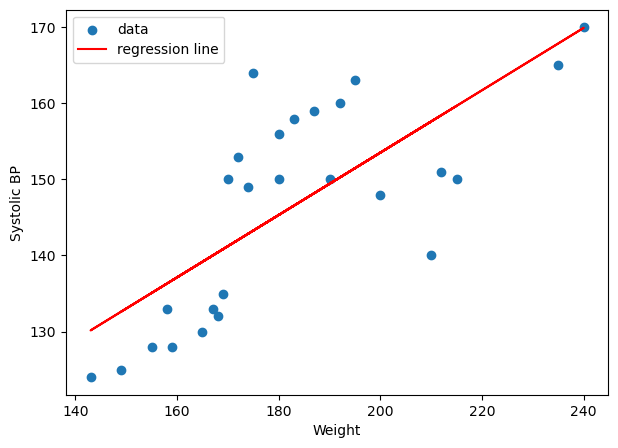
\includegraphics[width=0.6\textwidth]{./images/task1_output.png}
		\caption{Linear regression line fitting the given data points.}
		\label{fig:image1}
	\end{figure}
	
	\newpage
	\section*{Question 2: Multivariate Linear Regression Analysis (30 Marks)}
	This question examines the relationship between wear on a bearing \( y \), oil viscosity \( x_1 \), and load \( x_2 \).
	
	\subsection*{Given Data}
	The dataset includes the following values for oil viscosity (\( x_1 \)), load (\( x_2 \)), and bearing wear (\( y \)):
	
	\begin{center}
		\begin{tabular}{|c|c|c|}
			\hline
			\( x_1 \) & \( x_2 \) & \( y \) \\
			\hline
			1.6 & 851 & 293 \\
			15.5 & 816 & 230 \\
			22.0 & 1058 & 172 \\
			43.0 & 1201 & 91 \\
			33.0 & 1357 & 113 \\
			40.0 & 1115 & 125 \\
			\hline
		\end{tabular}
	\end{center}
	
	
	\subsection*{Part (a): Fit a Multivariate Linear Regression Model (10 Marks)}
	We want to fit a multivariate linear regression model of the form:
	\[
	y = b_0 x_1 + b_1 x_2 + b_2
	\]
	where \( b_0 \), \( b_1 \), and \( b_2 \) are the intercept and coefficients for the variables \( x_1 \) and \( x_2 \), respectively.
	
	We have equation \[XB=Y\] which X is matrix with columns \(x1\) and \(x2\) and we add third column with ones so it's coefficient will be the intercept, B is matrix of intercepts that we must find and Y is matrix with one column y.
	\[
	X=
	\begin{bmatrix}
		1.6 & 851 & 1 \\
		15.5 & 816 & 1 \\
		22.0 & 1058 & 1 \\
		43.0 & 1201 & 1 \\
		33.0 & 1357 & 1 \\
		40.0 & 1115 & 1 \\
	\end{bmatrix}
	\quad B=
	\begin{bmatrix}
		b_0 \\
		b_1 \\
		b_2
	\end{bmatrix} \quad Y=
	\begin{bmatrix}
		293 \\
		230 \\
		172 \\
		91 \\
		113 \\
		125 
	\end{bmatrix}
	\]
	
	But X is not squared mutrix we multiply transpose of matrix \(X\) from right to each side of the equation to create square matrix.(\(X^T X B = X^T Y\))
	
	\[
	\begin{bmatrix}
		5264.8 & 178309.6 & 155.1 \\
		178309.6 & 7036496 & 6398 \\
		155.1 & 6398 & 6.0
	\end{bmatrix}
	\begin{bmatrix}
		b_0 \\
		b_1 \\
		b_2
	\end{bmatrix} =
	\begin{bmatrix}
		20459.8 \\
		1021006 \\
		1024 
	\end{bmatrix}
	\]
	
	now if we convert this matrix to identity matrix the last column will represent the \( b_0 \), \( b_1 \), and \( b_2 \)
	
	
	\[
	\begin{bmatrix}
		5264.8 & 178309.6 & 155.1 & \vert & 20459.8 \\
		178309.6 & 7036496 & 6398 & \vert & 1021006 \\
		155.1 & 6398 & 6.0 & \vert & 1024
	\end{bmatrix}
	\]
	
	and after simplification we end up with this matrix
	
	\[
	\begin{bmatrix}
		1 & 0 & 0 & \vert & -3.8\\
		0 & 1 & 0 & \vert & -0.1\\
		0 & 0 & 1 & \vert & 372.2
	\end{bmatrix}
	\]
	
	\[
	b_0 \approx -3.8, \quad b_1 \approx -0.1, \quad b_2 \approx 372.2
	\]
	
	Thus, the regression model is:
	\[
	y = - 3.8 x_1 - 0.1 x_2 + 372.2
	\]
	
	\begin{figure}[h!]
		\centering
		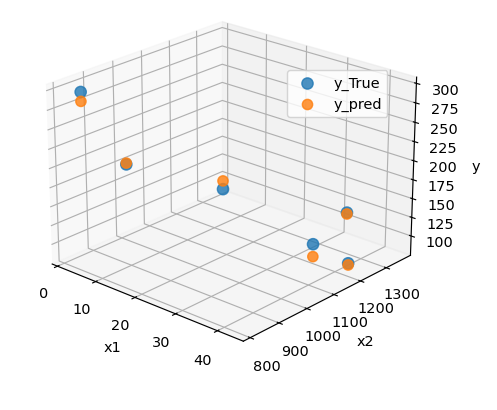
\includegraphics[width=0.6\textwidth]{./images/task2a_output.png}
		\caption{Multivariate Linear Regression}
		\label{fig:image2}
	\end{figure}
	
	
	\subsection*{Part (b): Predict Wear for \( x_1 = 25 \) and \( x_2 = 1000 \) (5 Marks)}
	To predict the wear \( y \) when \( x_1 = 25 \) and \( x_2 = 1000 \), we substitute these values into our model:
	
	\[
	y = 372.2 - 3.8 \cdot 25 - 0.1 \cdot 1000
	\]
	
	Calculating each term:
	\[
	y = 372.2 - 95 - 100
	\]
	\[
	y \approx 177.2
	\]
	
	Thus, the predicted wear \( y \) when \( x_1 = 25 \) and \( x_2 = 1000 \) is approximately \( 177.2 \).
	
	 \subsection*{Part (c): Fit a Multivariate Linear Regression Model with Interaction Term \( x_1 x_2 \) (15 Marks)}
	In this part, we add an interaction term \( x_1 x_2 \) to the model. The new model is:
	\[
	y = b_0 x_1 + b_1 x_2 + b_2 (x_1 x_2) + b_3
	\]
	
	like what we did in part (a) we first calculate \(X\),\(B\) and \(Y\) matrix and solve \(X B = Y\) equation.
	
	this time we add \(x_1 x_2\) as column three of matrix \(X\) and also we add it's coefficient to matrix \(B\)
	
	\[
	X=
	\begin{bmatrix}
		1.6 & 851 & 1361.6 & 1 \\
		15.5 & 816 & 12648 & 1 \\
		22.0 & 1058 & 23276 & 1 \\
		43.0 & 1201 & 51643 & 1 \\
		33.0 & 1357 & 44781 & 1 \\
		40.0 & 1115 & 44600 & 1 \\
	\end{bmatrix}
	\quad B=
	\begin{bmatrix}
		b_0 \\
		b_1 \\
		b_2 \\
		b_3
	\end{bmatrix} \quad Y=
	\begin{bmatrix}
		293 \\
		230 \\
		172 \\
		91 \\
		113 \\
		125 
	\end{bmatrix}
	\]
	
	now just like befor we must multiply the transpose of matrix \(X\) from right to both side of the equation and we end up with this equation
	
	\[
	\begin{bmatrix}
		5264.81 & 178309.6 & 6192716.56 & 155.1 \\
		178309.6 & 7036496 & 208625558 & 6398 \\
		6192716.56 & 208625558 & 7365095440 & 178309.6 \\
		155.1 & 6398 & 178309.6 & 6.0
	\end{bmatrix}
	\begin{bmatrix}
		b_0 \\
		b_1 \\
		b_2 \\
		b_3
	\end{bmatrix}
	\begin{bmatrix}
		20459.8 \\
		1021006 \\
		22646226.8 \\
		1024 
	\end{bmatrix}
	\]
	
	then just like befor we must convert matrix below to identity matrix
	
	\[
	\begin{bmatrix}
		5264.81 & 178309.6 & 6192716.56 & 155.1 & \vert & 20459.8 \\
		178309.6 & 7036496 & 208625558 & 6398 & \vert & 1021006 \\
		6192716.56 & 208625558 & 7365095440 & 178309.6 & \vert & 22646226.8 \\
		155.1 & 6398 & 178309.6 & 6.0 & \vert & 1024
	\end{bmatrix}
	\]
	
	finally we end up with this matrix
	
	\[
	\begin{bmatrix}
		1 & 0 & 0 & 0 & \vert & -7.6 \\
		0 & 1 & 0 & 0 & \vert & -0.22 \\
		0 & 0 & 1 & 0 & \vert & 0.004 \\
		0 & 0 & 0 & 1 & \vert & 483.96 \\
	\end{bmatrix}
	\]
	
	\[
	b_0 \approx -7.6, \quad b_1 \approx -0.22, \quad b_2 \approx 0.004 \quad b_3 \approx 483.96
	\]
	
	Thus, the regression model is:
	\[
	y = - 7.6 x_1 - 0.22 x_2 + 0.004 x_1 x_2 + 483.96
	\]
	
	\newpage
	\section*{Question 3}
	Given the regression problem with the prediction formula:
	\[
	o = w_0 + w_1 x_1 + w_1 x_1^3 + w_2 x_2 + w_2 x_2^3 + \dots + w_n x_n + w_n x_n^3,
	\]
	where \(O\) represents the predicted output, \(X\) is an \(n\)-dimensional vector, and \(W\) represents the weights \(w_1, w_2, \dots, w_n\), we will write the matrix form for this prediction using the data from \(m\) samples.
	
	\subsection*{Part (a): Matrix Form \(O = ZW\)}
	
	1. Define Matrices \(O\), \(Z\), and \(W\):
	
	Suppose we have \(m\) samples in our dataset. For each sample \(X^{(i)} = \begin{bmatrix} x_1^{(i)} & x_2^{(i)} & \dots & x_n^{(i)} \end{bmatrix}^T\), the output \(o^{(i)}\) is given by:
	\[
	o^{(i)} = w_0 + w_1 x_1^{(i)} + w_1 (x_1^{(i)})^3 + w_2 x_2^{(i)} + w_2 (x_2^{(i)})^3 + \dots + w_n x_n^{(i)} + w_n (x_n^{(i)})^3.
	\]
	
	2. Construct the Output Vector \(O\):
	
	Let \(O \in \mathbb{R}^m\) be the output vector for all \(m\) samples:
	\[
	O = \begin{bmatrix} o^{(1)} \\ o^{(2)} \\ \vdots \\ o^{(m)} \end{bmatrix}.
	\]
	
	3. Construct the Matrix \(Z\):
	
	We can express each prediction as a linear combination of the weights, represented by the matrix \(Z \in \mathbb{R}^{m \times (2n+1)}\) that includes both the linear and cubic terms for each feature. The matrix \(Z\) is constructed as follows:
	\[
	Z = \begin{bmatrix} 
		1 & x_1^{(1)} & (x_1^{(1)})^3 & x_2^{(1)} & (x_2^{(1)})^3 & \dots & x_n^{(1)} & (x_n^{(1)})^3 \\ 
		1 & x_1^{(2)} & (x_1^{(2)})^3 & x_2^{(2)} & (x_2^{(2)})^3 & \dots & x_n^{(2)} & (x_n^{(2)})^3 \\ 
		\vdots & \vdots & \vdots & \vdots & \vdots & \ddots & \vdots & \vdots \\ 
		1 & x_1^{(m)} & (x_1^{(m)})^3 & x_2^{(m)} & (x_2^{(m)})^3 & \dots & x_n^{(m)} & (x_n^{(m)})^3 
	\end{bmatrix}.
	\]
	
	4. Construct the Weight Vector \(W\):
	
	The weight vector \(W \in \mathbb{R}^{2n+1}\) includes the bias term \(w_0\) and the weights for both the linear and cubic terms of each feature:
	\[
	W = \begin{bmatrix} w_0 \\ w_1 \\ w_1 \\ w_2 \\ w_2 \\ \vdots \\ w_n \\ w_n \end{bmatrix}.
	\]
	
	5. Matrix Form of the Prediction:
	
	The prediction for all samples can be written in matrix form as:
	\[
	O = Z W.
	\]
	
	\subsection*{Part (b): Gradient Descent Relation for \(W\)}
	
	To obtain \(W\) using gradient descent, we need to update each weight \(w_i\) in \(W\) based on the error between the predicted output \(o^{(i)}\) and the actual target value for each sample. Let \(\hat{o}^{(i)}\) represent the actual target for the \(i\)-th sample, and let the loss function \(L\) be the mean squared error:
	\[
	L = \frac{1}{m} \sum_{i=1}^m (o^{(i)} - \hat{o}^{(i)})^2.
	\]
	
	The gradient of \(L\) with respect to \(w_i\) for \(1 \le i \le n\) is:
	\[
	\frac{\partial L}{\partial w_i} = \frac{2}{m} \sum_{j=1}^m (o^{(j)} - \hat{o}^{(j)}) \cdot \frac{\partial o^{(j)}}{\partial w_i}.
	\]
	
	Thus, the gradient descent update rule for each \(w_i\) is:
	\[
	w_i \leftarrow w_i - \eta \cdot \frac{\partial L}{\partial w_i},
	\]
	where \(\eta\) is the learning rate. This relation allows for iterative updates of each \(w_i\) to minimize the loss.
	
	\newpage
	\section*{Question 4 - Polynomial Basis Function}
	\subsection*{Polynomial Basis Function - part 1}
	In this part, we implemented linear basis function regression with polynomial basis functions to predict fuel efficiency (miles per gallon) from seven car features in the Auto MPG dataset. The dataset was divided into training (first 100 points) and testing (remaining points) sets. We trained polynomial models of degrees 1 to 10 and evaluated the models using Root Mean Square Error (RMS Error) for both the training and testing sets. The plot of RMS Error versus polynomial degree is shown in Figure \ref{fig:rms_error_vs_degree}.
	
	\subsection*{Steps and Key Code Snippets}
	
	\begin{itemize}
		\item \textbf{Data Loading and Preprocessing}: We loaded the dataset, dropped missing values, normalized the features and target to have zero mean and unit variance, and applied a permutation to randomize the data points. Here, only relevant features were selected, excluding the target variable \texttt{mpg}.
		
		\begin{verbatim}
			X_norm = (X - X.mean(axis=0)) / X.std(axis=0)
			y_norm = (y - y.mean(axis=0)) / y.std(axis=0)
		\end{verbatim}
		
		\item \textbf{Polynomial Feature Generation}: For each polynomial degree, we generated polynomial terms up to the specified degree for each of the seven input features. This was achieved by manually expanding \texttt{X\_train} and \texttt{X\_test} for each power up to the desired degree.
		
		\begin{verbatim}
			X_train_poly = np.hstack([X_train**deg for deg in range(degree + 1)])  
			X_test_poly = np.hstack([X_test**deg for deg in range(degree + 1)])
		\end{verbatim}
		
		\item \textbf{Model Training}: We used linear regression without regularization by directly solving the least squares equation to obtain model coefficients. The following code snippet shows how the coefficients were computed:
		
		\begin{verbatim}
			coef = np.linalg.lstsq(X_train_poly, y_train, rcond=None)[0]
		\end{verbatim}
		
		\item \textbf{Error Calculation}: After fitting the model, we computed the RMS Error for both training and testing sets and stored these values for each polynomial degree.
		
		\begin{verbatim}
			train_rmse = root_mean_squared_error(y_train, y_train_pred)
			test_rmse = root_mean_squared_error(y_test, y_test_pred)
		\end{verbatim}
	\end{itemize}
	
	\subsection*{Results and Observations}
	
	The plot of RMS Error versus polynomial degree is shown in Figure \ref{fig:rms_error_vs_degree}.
	
	\begin{figure}[h!]
		\centering
		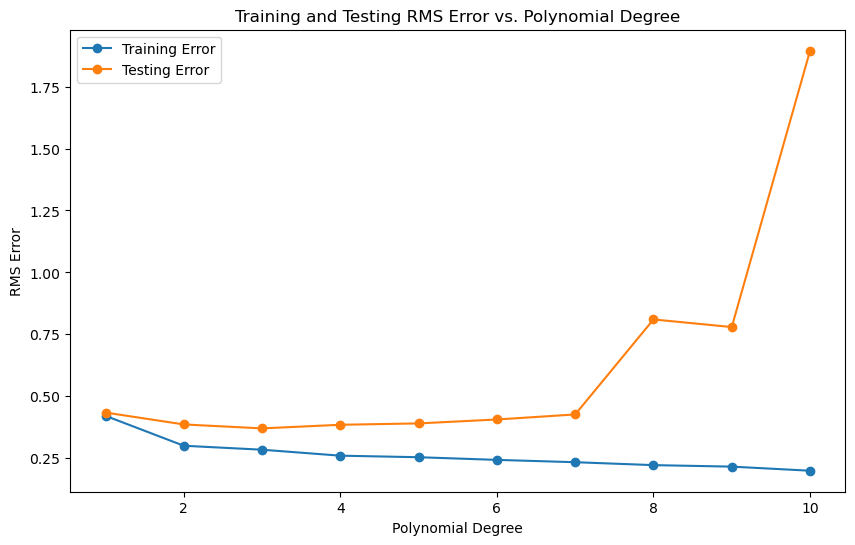
\includegraphics[width=0.6\textwidth]{./images/q4_part1.png}
		\caption{Training and Testing RMS Error vs. Polynomial Degree}
		\label{fig:rms_error_vs_degree}
	\end{figure}
	
	\paragraph{Comment:} In Figure \ref{fig:rms_error_vs_degree}, the training error consistently decreases as polynomial degree increases, indicating a better fit to the training data. However, the testing error initially remains stable but starts increasing significantly beyond degree 7, suggesting that higher-degree polynomials overfit the training data, capturing noise that does not generalize well to the testing data. we can see that polynomial with degree three is the best choice.
	
	\subsection*{Polynomial Basis Function - Part 2}
	
	In this part, we performed polynomial regression using only a single feature from the dataset—the normalized horsepower feature. We applied polynomial models of degrees 1, 4, and 10 to illustrate the effects of model complexity on the training and testing data. The results, shown in Figure \ref{fig:single_feature_polynomial_fits}, highlight the trade-offs between underfitting, a balanced fit, and overfitting.
	
	\subsection*{Steps and Key Code Snippets}
	
	\begin{itemize}
		\item \textbf{Feature Selection}: For this analysis, we used only the normalized horsepower feature (column index 2) as our input variable.
		\begin{verbatim}
			X_single_feature = X_norm[:, 2].reshape(-1, 1)  # Using "horsepower" feature
			X_train_single, X_test_single = X_single_feature[:100], X_single_feature[100:]
		\end{verbatim}
		
		\item \textbf{Polynomial Feature Transformation}: For each specified polynomial degree (1, 4, and 10), we generated polynomial features up to the selected degree.
		\begin{verbatim}
			for deg_single in range(1, degree+1):
				X_train_poly = np.hstack([X_train_poly, X_train_single**deg_single])
				X_test_poly = np.hstack([X_test_poly, X_test_single**deg_single])
		\end{verbatim}
		
		\item \textbf{Model Training}: We used linear regression without regularization by solving the least squares problem to obtain model coefficients.
		\begin{verbatim}
			coef = np.linalg.lstsq(X_train_poly, y_train, rcond=None)[0]
		\end{verbatim}
		
		\item \textbf{Visualization}: For each polynomial degree, we plotted the training and testing data points along with the polynomial fit. To produce a smooth curve, we evaluated the polynomial model on a dense set of points within the range of the training data.
		\begin{verbatim}
			X_range = np.linspace(X_train_single.min(), X_train_single.max(), 100).reshape(-1, 1)
		\end{verbatim}
	\end{itemize}
	
	\subsection*{Results and Observations}
	
	The polynomial regression fits for degrees 1, 4, and 10 are shown in Figure \ref{fig:single_feature_polynomial_fits}. 
	
	\begin{figure}[h!]
		\centering
		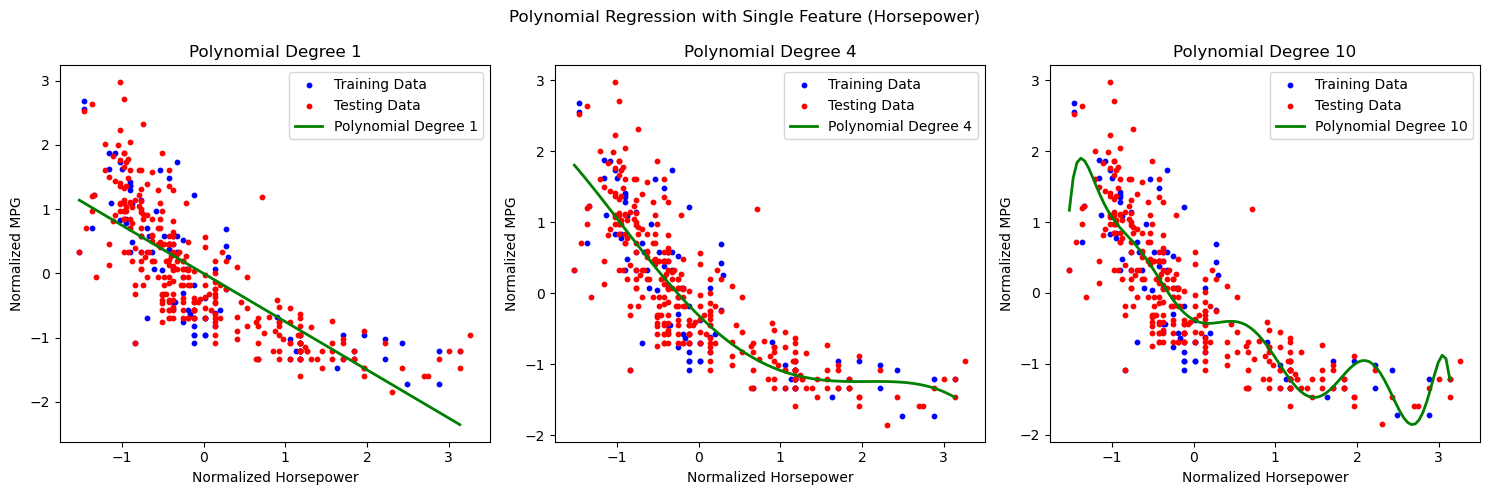
\includegraphics[width=\textwidth]{images/q4_part2.png} % Replace "image.png" with the actual filename
		\caption{Polynomial Regression with Single Feature (Horsepower)}
		\label{fig:single_feature_polynomial_fits}
	\end{figure}
	
	The figure illustrates the impact of increasing model complexity:
	
	\begin{itemize}
		\item \textbf{Polynomial Degree 1}: 
		\begin{itemize}
			\item This plot shows a linear regression model, representing a degree 1 polynomial.
			\item Blue dots correspond to the training data, and red dots represent the testing data.
			\item The green line represents the linear regression fit, indicating a negative trend. As horsepower increases, the MPG decreases, capturing the general direction of the relationship.
		\end{itemize}
		
		\item \textbf{Polynomial Degree 4}: 
		\begin{itemize}
			\item This plot shows a polynomial regression model of degree 4.
			\item The green curve fits the data more closely than the linear model, capturing a more nuanced relationship between horsepower and MPG.
			\item Degree 4 provides a balance between underfitting and overfitting, adapting to some of the nonlinear patterns in the data.
		\end{itemize}
		
		\item \textbf{Polynomial Degree 10}: 
		\begin{itemize}
			\item This plot shows a polynomial regression model of degree 10.
			\item The high-degree polynomial (green curve) exhibits significant fluctuations, indicating overfitting to the training data. This model captures noise rather than the underlying trend, which may result in poor generalization to new data.
		\end{itemize}
	\end{itemize}
	
	\paragraph{Conclusion:} This visualization highlights the trade-offs between model complexity and fit quality. A lower-degree polynomial (degree 1) underfits the data, while a very high-degree polynomial (degree 10) overfits. The degree 4 polynomial strikes a balance, capturing essential patterns in the data without excessive fluctuations.
	
	
	
	\subsection*{Polynomial Basis Function - Part 3}
	
	In Part 3, we applied polynomial regression with L2 regularization (ridge regression) using the normalized horsepower feature. The goal was to observe the effect of different regularization strengths on training and testing errors. We used a polynomial of degree 8 and varied the regularization parameter, $\lambda$, across a range of values. The results, shown in Figure \ref{fig:regularization_error_plot}, illustrate how regularization influences model performance.
	
	\subsection*{Steps and Key Code Snippets}
	
	\begin{itemize}
		\item \textbf{Feature Selection}: As in Part 2, we used only the normalized horsepower feature for this analysis.
		\begin{verbatim}
			X_single_feature = X_norm[:, 2].reshape(-1, 1)
			X_train_single, X_test_single = X_single_feature[:100], X_single_feature[100:]
		\end{verbatim}
		
		\item \textbf{Polynomial Feature Transformation with Regularization}: For each $\lambda$ value, we generated polynomial features up to degree 8 and applied L2 regularization using the normal equation:
		$$(X^T X + \lambda I) \theta = X^T y$$
		where $I$ is the identity matrix, with the bias term unregularized.
		\begin{verbatim}
			def fit_polynomial_l2(X, y, degree, lambda_value):
				X_poly = np.hstack([X**deg for deg in range(degree + 1)])
				I = np.eye(X_poly.shape[1])
				I[0, 0] = 0  # Do not regularize the bias term
				theta = np.linalg.solve(X_poly.T @ X_poly + lambda_value * I, X_poly.T @ y)
				return theta, X_poly
		\end{verbatim}
		
		\item \textbf{Error Calculation}: For each $\lambda$, we calculated the Root Mean Square Error (RMSE) for both the training and testing datasets.
		\begin{verbatim}
			train_rmse = root_mean_squared_error(y_train, y_train_pred)
			test_rmse = root_mean_squared_error(y_test, y_test_pred)
		\end{verbatim}
		
		\item \textbf{Visualization}: We plotted the training and testing errors against the regularization parameter $\lambda$ on a logarithmic scale.
		\begin{verbatim}
			plt.semilogx(lambdas, train_errors, label='Training Error', marker='o')
			plt.semilogx(lambdas, test_errors, label='Testing Error', marker='o')
		\end{verbatim}
	\end{itemize}
	
	 \subsection*{Results and Observations}
	
	The plot of training and testing errors versus the regularization parameter $\lambda$ is shown in Figure \ref{fig:regularization_error_plot}. 
	
	\begin{figure}[h!]
		\centering
		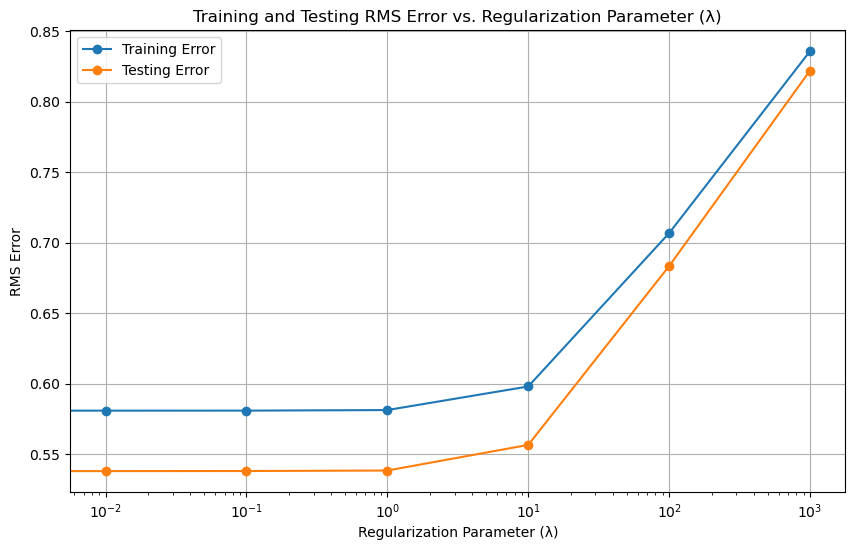
\includegraphics[width=0.6\textwidth]{images/q4_part3.png} 
		\caption{Training and Testing RMS Error vs. Regularization Parameter ($\lambda$)}
		\label{fig:regularization_error_plot}
	\end{figure}
	
	The figure illustrates the effect of increasing $\lambda$ on model performance:
	
	\begin{itemize}
		\item \textbf{Low $\lambda$ values ($10^{-2}$ to $10^{0}$)}:
		\begin{itemize}
			\item At low regularization values, the training error remains around 0.60, and the testing error hovers around 0.55.
			\item This range allows the model to fit the data without overfitting, maintaining a balance between bias and variance.
		\end{itemize}
		
		\item \textbf{High $\lambda$ values ($10^{1}$ and above)}:
		\begin{itemize}
			\item As $\lambda$ increases beyond $10^{1}$, both training and testing errors start to rise.
			\item At very high $\lambda$ values, such as $10^{3}$, the training error reaches around 0.85 and the testing error around 0.80, indicating a significant increase in both errors.
			\item High regularization values induce underfitting, as the model is overly constrained and unable to capture the complexity in the data.
		\end{itemize}
	\end{itemize}
	
	\paragraph{Conclusion:} This graph demonstrates how regularization affects model performance. Low values of $\lambda$ provide minimal regularization, preventing overfitting while achieving low errors. However, excessively high $\lambda$ values lead to underfitting, causing increased errors in both the training and testing datasets. This trade-off highlights the importance of selecting an appropriate regularization strength to balance bias and variance.
	
	
	\section*{Question 4 - Gaussian Basis Function Regression}
	
	In this question, we implement a Gaussian basis function regression model and evaluate its performance by varying the number of basis functions and applying L2 regularization. The Gaussian basis functions are defined as:
	\[
	\phi_j(x) = \exp\left(-\frac{\| x - \mu_j \|^2}{2s^2}\right)
	\]
	where each \(\mu_j\) is a randomly selected center from the training data, and \(s\) is set to 2.
	
	\subsection*{Experiment 1: Varying Number of Basis Functions}
	We use the first 100 points as training data and the rest as testing data. A Gaussian basis function regression model is fitted with an increasing number of basis functions (5, 15, 25, ..., 95) without regularization. The training and testing RMS errors are computed and plotted.
	
	Key Python code:
	\begin{lstlisting}[language=Python]
		# Define Gaussian basis functions
		def gaussian_basis(X, centers, s):
		  d2 = dist2(X, centers)
		  return np.exp(-d2 / (2 * s**2))
		
		# Loop over different numbers of basis functions
		for basis_size in basis_sizes:
		  centers = X_train[np.random.choice(X_train.shape[0], basis_size)]
		  X_train_gauss = gaussian_basis(X_train, centers, s)
		  theta = np.linalg.pinv(X_train_gauss) @ y_train
		  # Compute RMS errors for training and testing sets
	\end{lstlisting}
	
	\begin{figure}[!h]
		\centering
		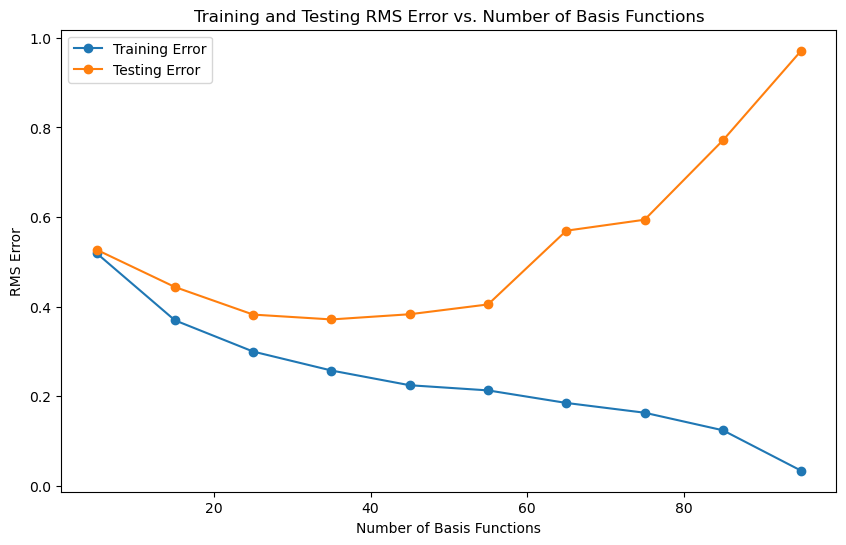
\includegraphics[width=0.6\textwidth]{images/q4_par4a.png}
		\caption{Training and Testing RMS Error vs. Number of Basis Functions}
		\label{fig:basis_functions_plot}
	\end{figure}
	
	\paragraph{Observation:}
	As shown in Figure \ref{fig:basis_functions_plot}, increasing the number of basis functions reduces training error but does not significantly affect testing error, indicating overfitting as the model becomes more complex.
	
	\subsection*{Experiment 2: L2-Regularized Regression}
	Next, we apply L2 regularization with 90 basis functions, varying the regularization parameter \(\lambda\) over the values \(0, 0.01, 0.1, 1, 10, 100, 1000\). The regularization parameter controls model complexity by penalizing large coefficients.
	
	Key Python code:
	\begin{lstlisting}[language=Python]
		# Apply L2 regularization with different values of lambda
		for lambda_value in lambdas:
		  I = np.eye(X_train_gauss.shape[1])
		  theta = np.linalg.solve(X_train_gauss.T @ X_train_gauss 
		                          + lambda_value * I, 
		                          X_train_gauss.T @ y_train)
		  # Compute RMS errors for training and testing sets
	\end{lstlisting}
	
	\begin{figure}[!h]
		\centering
		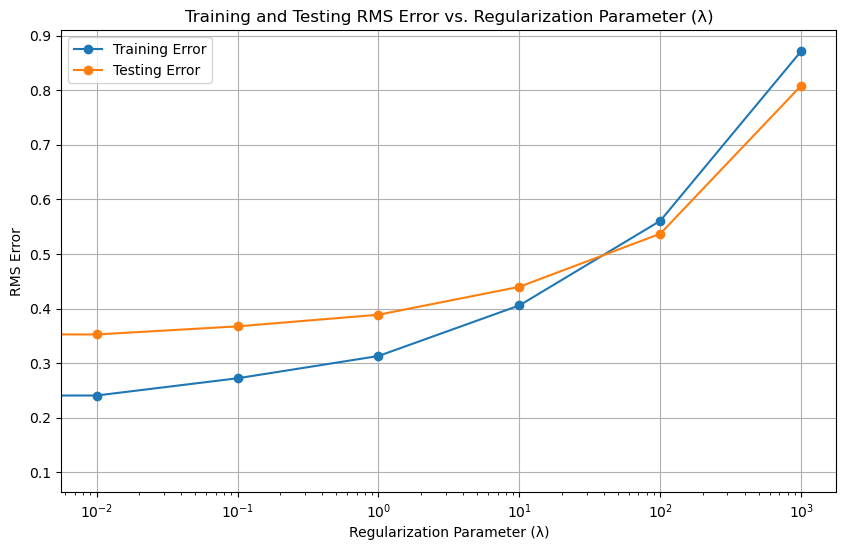
\includegraphics[width=0.6\textwidth]{images/q4_par4b.png}
		\caption{Training and Testing RMS Error vs. Regularization Parameter (\(\lambda\))}
		\label{fig:regularization_plot}
	\end{figure}
	
	\paragraph{Observation:}
	In Figure \ref{fig:regularization_plot}, the training RMS error increases as \(\lambda\) increases, while the testing error remains relatively stable. Small values of \(\lambda\) lead to lower training error but may cause overfitting, whereas larger values encourage underfitting due to excessive regularization.
	
	\subsection*{Conclusion}
	From these experiments, we observe that:
	\begin{itemize}
		\item Increasing the number of basis functions improves the fit to training data but increases overfitting risk, as seen from high testing error.
		\item L2 regularization helps control model complexity, with larger values of \(\lambda\) reducing overfitting but possibly leading to underfitting.
	\end{itemize}
	The choice of basis functions and regularization parameter should balance bias and variance to optimize model generalization.
	
	\newpage
	\section*{Question 5: Linear Regression with Basis Function}
	
	In this question, we are given a one-dimensional dataset contained in the file \texttt{q4\_dataset.csv}. We will visualize the dataset and apply a linear regression model with a quadratic basis function to improve the model's fit.
	
	\subsection*{Part (a): Basis Function}
	To fit a linear regression model on the dataset, we will utilize a quadratic basis function that maps the input features \( X \) to a higher-dimensional space. The transformation is defined as:
	\[
	\phi(X) = \begin{bmatrix}
		1 \\
		X \\
		X^2
	\end{bmatrix}
	\]
	This transformation allows the linear regression model to capture non-linear relationships between the input features and the labels.
	
	\subsection*{Part (b): Implementation}
	
	\subsubsection*{Data Visualization}
	We start by visualizing the dataset, where \( X \) serves as input features and \( Y \) as labels. The following code snippet demonstrates how to visualize the data points in a two-dimensional space:
	
	
	\begin{figure}[!h]
		\centering
		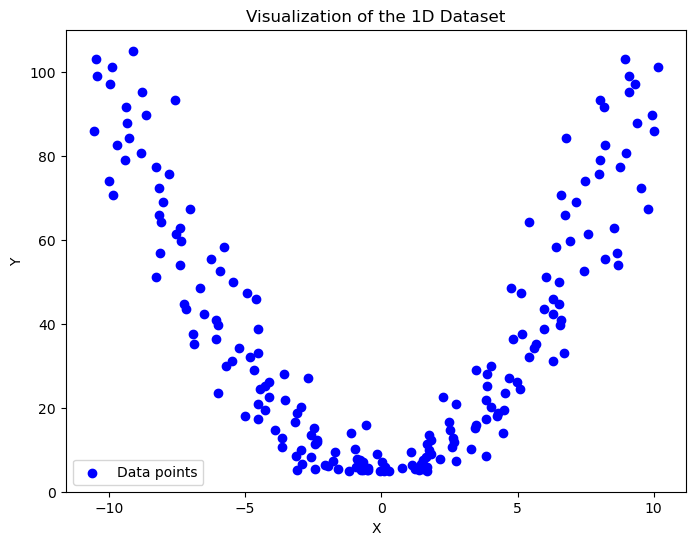
\includegraphics[width=0.5\textwidth]{images/q5_data.png}
		\caption{Training data for question five (\(\lambda\))}
		\label{fig:q5_data}
	\end{figure}
	
	\subsubsection*{Data Splitting and Model Training}
	Next, we divide the dataset into training (80\%) and testing (20\%) subsets using random sampling. The model is then trained using the normal equation to find the optimal parameters:
	\begin{lstlisting}[language=Python]
		# Split the dataset into training (80%) and testing (20%) sets
		np.random.seed(0)  # For reproducibility
		indices = np.random.permutation(len(X))
		train_size = int(0.8 * len(X))
		train_indices, test_indices = indices[:train_size], indices[train_size:]
		
		X_train, Y_train = X[train_indices], Y[train_indices]
		X_test, Y_test = X[test_indices], Y[test_indices]
		
		# Transform features using the quadratic basis function
		X_train_basis = quadratic_basis(X_train)
		
		# Train the linear regression model using the normal equation
		theta = np.linalg.inv(X_train_basis.T @ X_train_basis) @ X_train_basis.T @ Y_train
	\end{lstlisting}
	
	\subsubsection*{Model Evaluation}
	We compute the Mean Squared Error (MSE) on the test set to evaluate the model's performance:
	\begin{lstlisting}[language=Python]
		# Make predictions on the test set
		Y_test_pred = X_test_basis @ theta
		
		# Compute Mean Squared Error (MSE)
		mse = np.mean((Y_test - Y_test_pred)**2)
		print(f"Mean Squared Error on the Test Set: {mse:.4f}")
	\end{lstlisting}
	
	\subsubsection*{Model Visualization}
	Finally, we visualize the training data, test data, and model predictions:
	
	
	\begin{figure}[!h]
	\centering
	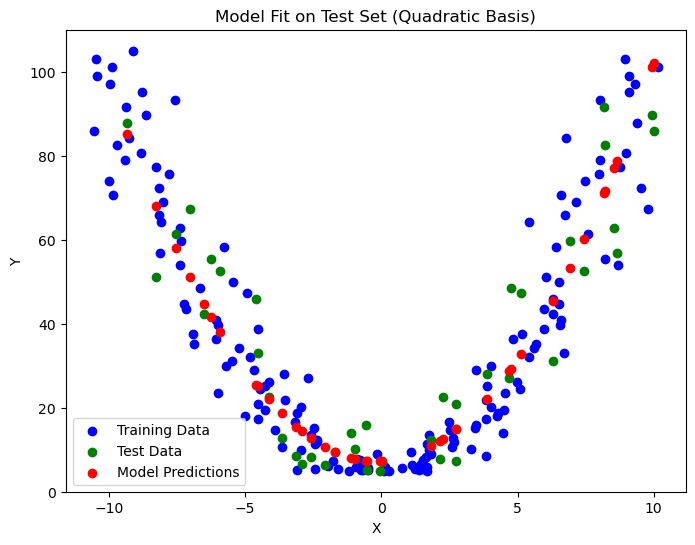
\includegraphics[width=0.5\textwidth]{images/q5_predicted.png}
	\caption{Training data for question five (\(\lambda\))}
	\label{fig:q5_predicted}
	\end{figure}
	
	\subsection*{Results}
	The Mean Squared Error on the test set was computed to be approximately: 
	\[
	\text{MSE} \approx [112.78]
	\]
	This indicates how well the model performed on unseen data.
	
	
	\newpage
	\section*{Question 6: Predicting Abalone Age}
	
	The Abalone dataset, obtained from the UCI Machine Learning Repository, is used to predict the age of abalones based on physical measurements. The primary task is to predict the number of rings, which indicates the age. This study explores the effectiveness of different kernel functions in a regression model to minimize the Mean Squared Error (MSE) between predicted and actual ring counts.
	
	\subsection*{Data Preparation}
	The dataset includes several continuous features (length, diameter, height, etc.) and a categorical feature for gender, which was removed to simplify the analysis. The continuous features were standardized to improve model stability.
	
	\subsection*{Methodology}
	We evaluated four different kernel functions in predicting the abalone rings:
	\begin{enumerate}
		\item Linear Regression
		\item Polynomial Kernel (Degree 2 and 3)
		\item RBF Kernel (with different $\gamma$ values)
	\end{enumerate}
	
	The models were trained on 80\% of the dataset, with the remaining 20\% reserved for testing. MSE was calculated for both the training and testing sets to assess model performance.
	
	\subsection*{Linear Regression}
	Implemented as follows:
	\begin{verbatim}
		def linear_regression(X, y):
		  X_b = np.c_[np.ones((X.shape[0], 1)), X]
		  theta_best = np.linalg.inv(X_b.T.dot(X_b)).dot(X_b.T).dot(y)
		  return theta_best
	\end{verbatim}
	The resulting MSE for both training and testing sets were calculated.
	
	\subsection*{Polynomial Regression}
	For polynomial regression, polynomial features were generated up to the specified degree:
	\begin{verbatim}
		def polynomial_features(X, degree):
		  return np.column_stack([X ** d for d in range(1, degree + 1)])
		
		def polynomial_regression(X, y, degree):
		  X_poly = polynomial_features(X, degree)
		  X_poly_b = np.c_[np.ones((X_poly.shape[0], 1)), X_poly]
		  theta_best = np.linalg.inv(X_poly_b.T.dot(X_poly_b)).dot(X_poly_b.T).dot(y)
		  return theta_best
	\end{verbatim}
	
	\subsection*{RBF Kernel Regression}
	Implemented with gamma tuning:
	\begin{verbatim}
		def rbf_kernel(x1, x2, gamma):
		  sq_dists = np.sum(x1**2, axis=1).reshape(-1, 1) + np.sum(x2**2, axis=1) - 2 * np.dot(x1, x2.T)
		  return np.exp(-gamma * sq_dists)
		
		def rbf_regression(X_train, y_train, X_test, gamma):
		  K_train = rbf_kernel(X_train, X_train, gamma)
		  K_test = rbf_kernel(X_test, X_train, gamma)
		  alpha = np.linalg.inv(K_train + 1e-8 * np.eye(K_train.shape[0])).dot(y_train)
		  y_pred_train = K_train.dot(alpha)
		  y_pred_test = K_test.dot(alpha)
		  return y_pred_train, y_pred_test
	\end{verbatim}
	Different values of $\gamma$ were tested to find the best fit.
	
	\subsection*{Results and Analysis}
	\subsection*{MSE Comparison of Different Kernel Functions}
	\begin{figure}[h!]
		\centering
		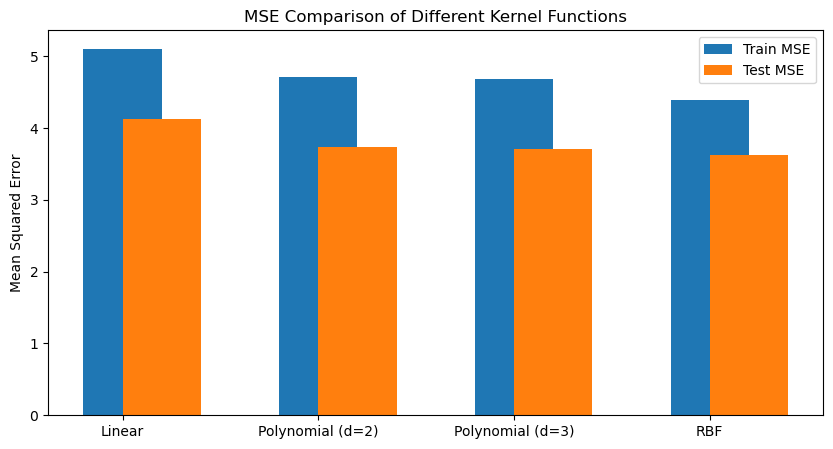
\includegraphics[width=0.6\textwidth]{images/q6_mse_compare.png}
		\caption{Comparison of Train and Test MSE for Different Kernel Functions}
		\label{fig:mse_comparison}
	\end{figure}
	
	Figure \ref{fig:mse_comparison} presents the MSE for each kernel function. The x-axis shows the models: Linear, Polynomial (degree 2), Polynomial (degree 3), and RBF, while the y-axis represents the MSE values. The blue bars indicate Train MSE, and the orange bars indicate Test MSE.
	
	\paragraph*{Observations:}
	\begin{itemize}
		\item \textbf{Linear Kernel:} Train MSE $\approx 5.1$, Test MSE $\approx 4.1$
		\item \textbf{Polynomial Kernel (degree=2 and degree=3):} Train MSE $\approx 4.7$, Test MSE $\approx 3.7$
		\item \textbf{RBF Kernel:} Train MSE $\approx 4.4$, Test MSE $\approx 3.6$
	\end{itemize}
	
	\subsection*{Actual vs. Predicted Rings Using RBF Kernel}
	\begin{figure}[h!]
		\centering
		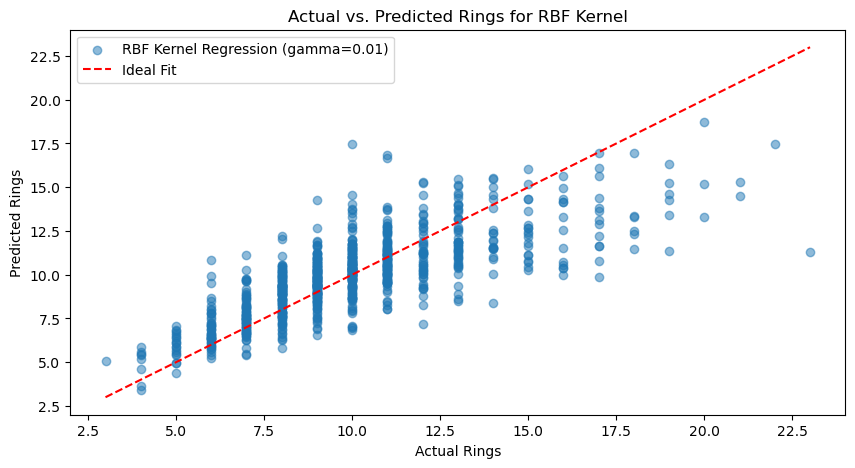
\includegraphics[width=0.6\textwidth]{images/q6_ActualVsPredicted.png}
		\caption{Actual vs. Predicted Rings for RBF Kernel (gamma=0.01)}
		\label{fig:actual_vs_predicted_rbf}
	\end{figure}
	
	Figure \ref{fig:actual_vs_predicted_rbf} shows the scatter plot of actual versus predicted ring counts using the RBF Kernel Regression model with $\gamma=0.01$. The x-axis represents actual ring counts, while the y-axis shows predicted ring counts.
	
	\subsection*{Conclusion}
	This analysis compared the performance of different kernel functions on the Abalone dataset using Mean Squared Error as the evaluation metric. The RBF kernel ($\gamma = 0.01$) provided a good balance between train and test MSE, suggesting these models generalize well. These findings suggest RBF kernels may be preferable for this dataset and task.

\end{document}
